\documentclass[10pt,english]{article}
\usepackage[T1]{fontenc}
\usepackage[latin9]{inputenc}
\usepackage{geometry}
\geometry{verbose,tmargin=1.5in,bmargin=1.5in,lmargin=1.5in,rmargin=1.5in}
\usepackage{amsthm}
\usepackage{amsmath}
\usepackage{amssymb}

\makeatletter
\usepackage{enumitem}
\newlength{\lyxlabelwidth}

\usepackage[T1]{fontenc}
\usepackage{ae,aecompl}

%\usepackage{txfonts}

\usepackage{microtype}

\usepackage{calc}
\usepackage{enumitem}
\setenumerate{leftmargin=!,labelindent=0pt,itemindent=0em,labelwidth=\widthof{\ref{last-item}}}

\usepackage{tikz}
\makeatother

\usepackage{babel}
\begin{document}
\noindent \begin{center}
\textbf{\large{}MATH 146 - Assignment 1}\\
\textbf{\large{}Chris Ji 20725415}
\par\end{center}{\large \par}
\medskip{}

\begin{enumerate}
\pagebreak\item Observe that $L_1$ has three perfect matchings: choosing the vertical lines, the horizontal lines, and the diagonals. 

\pagebreak\item Say there is some vertex $v$ such that it is not $M-$saturated for some maximum matching $M$ of $G$. Note we can work with just one matching, because every possible maximum matching such that $v$ is not saturated has the following property. Since $G$ is connected, and $M$ is a maximum matching, all of $v$'s neighbours much be saturated. Let $u$ be a neighbour of $v$ that is saturated by some edge $e$, connecting it to another vertex. Now observe the matching $M'$ of $G$ by removing $e$ from the matching, and adding the edge $e'=\{u,v\}$. This is still a valid matching, as $v$ was previously unsaturated, and $u$ is still saturated. $M'$ has the same number of edges as $M$, and so is also a maximum matching of $G$. 


\pagebreak\item Since $P=\{u=u_0,u_1,\ldots,u_n=v\}$ is an alternating path of even length, we know that $v$ is $M-$saturated. Also, there are $\frac{n}{2}$ matchings. Consider another matching, $M'$, such that every edge not in $M$ in $P$ is in $M'$, and every edge in $M$ in $P$ is not in $M'$. Then this results in a matching with the exact same amount of matchings, and hence it is also a maximum matching, and notice that $v$ is $M'$-unsaturated. 


\pagebreak\item \begin{enumerate}
    \item Note that trees are all bipartite. Let $T$ be bipartitioned by $A$ and $B$. Since every edge connects a vertex in $A$ to a vertex in $B$, we can find two vertex covers: exactly the vertices in $A$ and $B$. The smallest one is clearly the $\text{min}\{|A|,|B|\}$, and the minimum between these two bipartitions of $T$ is clearly at most $\left\lfloor\frac{n}{2}\right\rfloor$, and so the size of a vertex cover is at most $\left\lfloor\frac{n}{2}\right\rfloor$
    
    \item Suppose $T$ has two distinct perfect matchings, $M$ and $M'$. If they are distinct, then the union of the edge sets will give us a graph where every component is either 2 vertices connected by a single edge (ie. the edge is shared between $M$ and $M'$), or the edges in a path are distinct between $M$ and $M'$. But if all edges are distinct between $M$ and $M'$ in this path, it will eventually close on itself, and we obtain a cycle. This is contradictory to the fact that $T$ is a tree, and so $M$ and $M'$ can not be distinct, and so $T$ has at most 1 perfect matching. 
\end{enumerate}



\pagebreak\item \begin{enumerate}
    \item \leavevmode\vadjust{\vspace{-\baselineskip}}\newline
    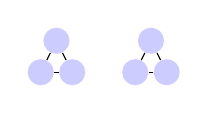
\begin{tikzpicture}
  [scale=.8,auto=left,every node/.style={circle,fill=blue!20},baseline]
  \node (n1) at (-1,0)  {};
  \node (n2) at (-0.5,0)  { } ;
  \node (n3) at (0.5,0)    {} ;
  \node (n4) at (1,0)  {} ;
  \node (n5) at (-0.75,0.5)  {} ;
  \node (n6) at (0.75,0.5)   {} ;
  
  \foreach \from/\to in {n1/n2,n1/n5,n5/n2,n3/n4,n3/n6,n6/n4}
    \draw (\from) -- (\to);
\end{tikzpicture} Observe that a maximum matching is of size 2, and a minimum cover is of size 4. 
    \item Consider any maximum matching $M$ of a graph $G$. Clearly we can take all ends of edges from a maximum matching to get a vertex cover, with the size of this being $2|M|$ (2 vertices per edge, every edge is distinct). Consider if this wasn't a minimum cover: then there is an edge $e$ that has both ends not in the matching. But then $M$ is not a maximum matching, as we can add the edge $e$ to it. So we can always find a vertex cover of size $2|M|$. Clearly a minimum vertex cover's size will be at most the size of any other vertex cover, in this case $2|M|$, and so a minimum vertex cover will always have size at most twice the size of a matching.
\end{enumerate}
\end{enumerate}

\end{document}
